\documentclass[12pt]{aghdpl}
\usepackage{graphicx}
\usepackage{float}
\usepackage[dvipsnames]{xcolor}
% \documentclass[language=en,11pt]{aghdpl}  % praca w języku angielskim

%---------------------------------------------------------------------------

\author{Tomasz Mikurda}
\shortauthor{T. Mikurda}

%\titlePL{Przygotowanie bardzo długiej i pasjonującej pracy dyplomowej w~systemie~\LaTeX}
%\titleEN{Preparation of a very long and fascinating bachelor or master thesis in \LaTeX}

\titlePL{Aplikacja webowa wspomagająca obsługę społecznościowej gry wojenno-strategicznej}
\titleEN{A web application for supporting the management of a strategy war game}


\shorttitlePL{Aplikacja webowa wspomagająca obsługę społecznościowej gry wojenno-strategicznej} % 
\shorttitleEN{A web application for supporting the management of a strategy war game}


% Dopuszczalne wartości[1,2]:
% * "Projekt dyplomowy" - na koniec studiów I stopnia
% * "Praca dyplomowa" - na koniec studiów II stopnia
% [1] Zasady dyplomowania w roku akademickim 2020/2021 (Decyzja Dziekana WEAIiIB nr 16/2020 z dnia 9 grudnia 2020 roku)
% [2] Załącznik nr 1a) do Decyzji nr 16/2020 Dziekana Wydziału EAIiIB z dnia 09 grudnia 2020 r.
\thesistype{Projekt dyplomowy}
%\thesistype{Master of Science Thesis}

\supervisor{dr inż. Grzegorz Rogus}
%\supervisor{Paweł Kłeczek, PhD}

\degreeprogramme{Automatyka i Robotyka}
%\degreeprogramme{Automatics and Robotics}

\date{2024}

%\department{Katedra Informatyki Stosowanej}
%\department{Department of Applied Computer Science}

\faculty{Wydział Elektrotechniki, Automatyki, Informatyki i Inżynierii Biomedycznej}
%\faculty{Faculty of Electrical Engineering, Automatics, Computer Science and Biomedical Engineering}

\acknowledgements{Serdecznie dziękuję \dots tu ciąg dalszych podziękowań np. dla promotora, żony, sąsiada itp.}


\begin{document}

	\titlepages
	\RedefinePlainStyle
	
	\setcounter{tocdepth}{2}
	\tableofcontents
	\clearpage
	
	\chapter{Wstęp}
\label{cha:wstep}

    Gra „War Thunder” tworzona przez firmę Gaijin Entertainment posiada ponad 70 milionów użytkowników na wielu platformach, z czego każdym momencie zalogowanych jest ponad 100 tysięcy aktywnych graczy. Gra skupia się na pojedynkach wszelkiego rodzaju pojazdów wojskowych. W ogólnej społeczności graczy wytworzyło się wiele mniejszych grup skupiających się na poszczególnych elementach gry, w tym także oczekujących bardziej strategicznego podejścia do rozgrywki. Sama gra nie oferuję takich rozwiązań, dlatego gracze tworzą własne systemy wykraczające poza samą rozgrywkę.

    Większe społeczności często tworzą swoje własne skomplikowane systemy dopełniające rozgrywkę pod różnymi względami. Przykładowo takie systemy mogą zawierać podział na drużyny z własnymi listami dostępnych pojazdów, niezależną od samej gry ekonomię i różne związane z nią rozwiązania. „War Thunder” posiada rozbudowany system niestandardowych gier własnych z którego korzystają wszystkie takie grupy, jednak poza samą rozgrywką, gra nie zapewnia im żadnego wsparcia.
    
	Zwykle stosuje się do tego ogólnodostępne narzędzia „pracy grupowej”, takie jak google sheets lub office 365, jednak wraz ze wzrostem liczby uczestników to także staje się problematyczne. Ze względu na swoją charakterystykę działania, otwarte dokumenty niosą ze sobą wiele zagrożeń związanych z bezpieczeństwem, prywatnością czy trwałością danych. Ze względu na społecznościową naturę problemu, ogólny dostęp do danych musi być publiczny, co naraża nas na zagrożenia związane z kradzieżą własności intelektualnej przez „złych aktorów”. Dostęp do edycji takich dokumentów zwykle może mieć tylko wąska grupa zaufanych członków społeczności, na którą spada odpowiedzialność za ich wypełnianie, aktualizowanie i utrzymanie. Takie osoby są także narażone na utratę anonimowości i prywatności, ponieważ serwisy udostępniające takie usługi często wymagają rejestracji przy pomocy danych osobowych i adresów e-mail, które są następnie widoczne dla pozostałych użytkowników.				
 
 	Rozwiązaniem tych problemów często jest stworzenie dedykowanej aplikacji obsługującej kwestie związane ze zbieraniem, przetwarzaniem i zapisem wszelakich potrzebnych danych i wykonującej inne przydatne zadania. Przyjmuje ona najczęściej formę aplikacji internetowej.

    \begin{figure}
        \centering
        \includegraphics[width=0.8\textwidth]{imgs/WTSS.png}
        \caption{Zrzut ekranu z rozgrywki}
    \end{figure}

    \begin{figure}
        \centering
        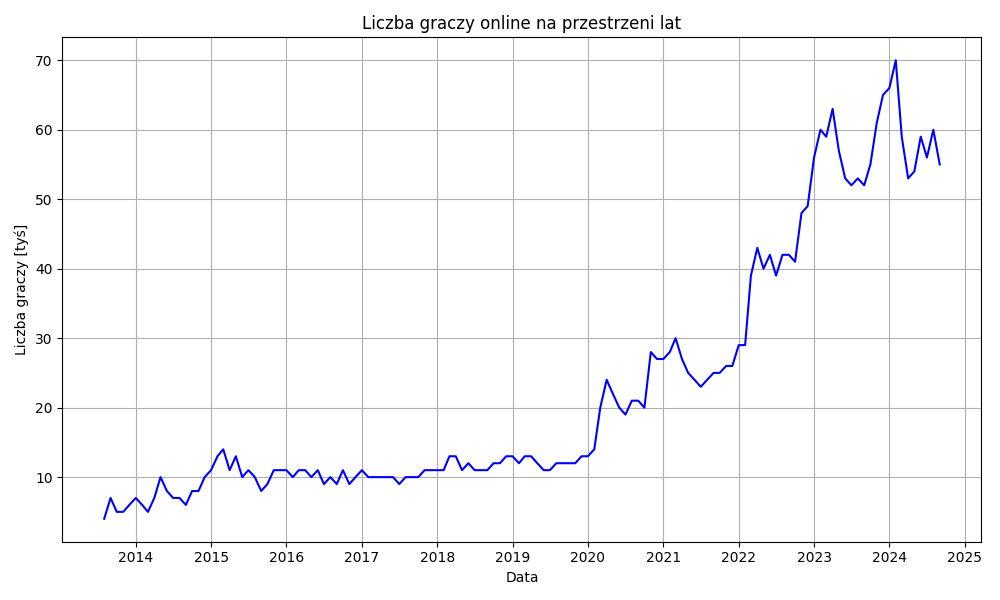
\includegraphics[width=0.8\textwidth]{imgs/wykres_graczy.png}
        \caption{Wykres liczby graczy online w jednej chwili
            Na wykresie znajdują się jedynie dane z platformy Steam, dlatego są one mocno niedoszacowane. Wydawca podaje dane na poziomie 100 – 150 tysięcy graczy online
            (źródło: steamcharts.com)}
    \end{figure}

.

    \newpage

%---------------------------------------------------------------------------

    \section{Cel i zakres pracy }
    \label{sec:celePracy}

    	Celem tej pracy jest stworzenie aplikacji, która zautomatyzuje procesy zbierania, zarządzania i dystrybucji danych w społeczności skupionej wokół organizacji własnych gier i turniejów z zewnętrznym systemem ekonomii i zarządzania drużynami. Aplikacja ta pozwoli na zwiększenie efektywności pracy moderatorów, poprzez uproszczenie lub całkowite uwolnienie ich z części obowiązków obsługi społeczności, dzięki rozproszeniu ich na każdego aktywnego uczestnika. Aplikacja pozwoli w kontrolowany sposób zamieszczać dane o rozgrywkach każdemu ich uczestnikowi i da każdej drużynie możliwość bezpośredniego kontrolowania własnych zasobów. System pozwoli także wprowadzić rozwiązania i plany nie możliwe do realizacji przy pomocy aktualnych rozwiązań opartych o google sheets.\\

        Główne Funkcje aplikacji:
        \begin{itemize}
            \item Zapewnienie miejsca dla udostępniania danych o dostępnych pojazdach.
            \item Możliwość zakupu, sprzedaży i ulepszeń pojazdów.
            \item Umożliwienie tworzenia i zarządzania drużynami.
            \item System planowania rozgrywek między drużynowych.
            \item Automatyczne obliczanie wynagrodzeń na podstawie wyniku rozgrywek.
            \item Zapisywanie i wizualizowanie wszystkich transakcji drużyn.
        \end{itemize}%[1)]

        Elementy aplikacji:
        \begin{itemize}
            \item Baza danych - PostgreSQL
            \item Backend - Python
            \item Frontend - Javascript
            \item Konteneryzacja - Docker
            \item Deployment i hosting - AWS.
        \end{itemize}%[1)]

%---------------------------------------------------------------------------

\section{Zawartość pracy}
\label{sec:zawartoscPracy}

W rozdziale~\ref{cha:Tech} przedstawiono opis wykorzystanych w pracy technologii

Jeszcze kilka odnośników do bibliografii \cite{PeDa04,BuDo03}.
	\chapter{Opis Technologii}
\label{cha:Tech}

W rozdziale tym przedstawiono informację o technologiach wykorzystanych przy tworzeniu aplikacji.

%---------------------------------------------------------------------------

\section{PostgreSQL}
\label{sec:PSQL}

    PostgreSQL jest jednym z najpopularniejszych systemów bazo-danowych i numerem jeden wśród rozwiązań open-source. 

    \begin{table}[H]
    \begin{center}
        \caption{Ranking najpopularniejszych systemów bazo-danowych wg. db-engines.com \cite{DbEg01}}
        \begin{tabular}{|c|c|c|c|}
            \hline
            Ranking & Nazwa & Wynik & Zmiana \\
            \hline
            1 & Oracle  & 1309.45 & \textcolor{Green}{+22.85} \\
            \hline
            2 & My SQL & 1022.76 & \textcolor{Red}{-6.73}  \\
            \hline
            3 & Microsoft SQL Server & 802.09 & \textcolor{Red}{-5.67} \\
            \hline
            4 & PostgreSQL & 652.16 &  \textcolor{Green}{+7.80} \\
            \hline
            5 & MongoDB & 405.21 & \textcolor{Red}{-5.02} \\
            \hline
        \end{tabular}
        \end{center}
    \end{table}

    Ranking jest wyliczana na podstawie wielu czynników, takich jak dane z Google Trends, pytań na Stack Overflow lub ofert pracy. Z danych wynika że PostgreSQL jest najbardziej popularnych rozwiązaniem open-source, i jako jedyny poza widocznym liderem - Oracle nie traci na popularności.

    Postgres jest systemem relacyjnym, skupionym na zgodnościa ze standarem SQL. 


%---------------------------------------------------------------------------

\section{Python}
\label{sec:Python}

\subsection{Django}

%---------------------------------------------------------------------------

\section{JavaScript}
\label{sec:JS}

\subsection{Vue}

%---------------------------------------------------------------------------

\section{Docker}
\label{sec:Docker}


%---------------------------------------------------------------------------

\section{AWS}
\label{sec:AWS}

\subsection{ECS}
	\chapter{Implementacja}
\label{cha:Imp}

W rozdziale przedstawiam Implementację aplikacji. 

%---------------------------------------------------------------------------

\section{Baza danych}
\label{sec:baza}


%---------------------------------------------------------------------------

\section{Backend}
\label{sec:back}

\subsection{}

%---------------------------------------------------------------------------

\section{Frontend}
\label{sec:front}

\subsection{}

%---------------------------------------------------------------------------

\section{Konteneryzacja}
\label{sec:kont}


%---------------------------------------------------------------------------

\section{Deploy}
\label{sec:deploy}

\subsection{}
	
	% itd.
	% \appendix
	% \include{dodatekA}
	% \include{dodatekB}
	% itd.
	
	\printbibliography

\end{document}
